\documentclass[preprint]{aastex}

\usepackage{verbatim}
\usepackage{color}
% A comment block

%\newcommand{\comment}[1]{}

% For color
\newcommand{\mpname}[1]{#1_color.eps}
\newcommand{\clraitoff}{red}
\newcommand{\lumblack}{(black)}
\newcommand{\lumblue}{(blue)}
\newcommand{\lumred}{(red)}
\newcommand{\vdisred}{(red-dashed curve)}
\newcommand{\vdisblue}{(blue-solid curve)}

% For bw
%\newcommand{\mpname}[1]{#1.eps}
%\newcommand{\clraitoff}{}
%\newcommand{\lumblack}{}
%\newcommand{\lumblue}{}
%\newcommand{\lumred}{}
%\newcommand{\vdisred}{(dashed curve)}
%\newcommand{\vdisblue}{(solid curve)}

\newcommand{\umag}{$u$}
\newcommand{\gmag}{$g$}
\newcommand{\rmag}{$r$}
\newcommand{\imag}{$i$}
\newcommand{\zmag}{$z$}
\newcommand{\gmr}{$g-r$}



\newcommand{\gammat}{$\gamma_T$}
\newcommand{\gammacross}{$\gamma_\times$}
\newcommand{\deltasig}{$\Delta \Sigma$}
\newcommand{\deltaplus}{$\Delta \Sigma_+$}
\newcommand{\deltacross}{$\Delta \Sigma_\times$}
\newcommand{\deltarho}{$\Delta \rho$}
\newcommand{\movr}{$M(<r)$}
\newcommand{\sigmacrit}{$\Sigma_{crit}$}

\newcommand{\photoz}{photo-z}
\newcommand{\photozs}{photo-zs}

\newcommand{\tlum}{$L^{tot}$}
\newcommand{\tngal}{$N_{gal}^{tot}$}

\newcommand{\lstarlim}{$0.4 L_*$}
\newcommand{\lvir}{$L_{200}$}
\newcommand{\nvir}{$N_{200}$}
\newcommand{\rvir}{$r_{200}^{gals}$}

\newcommand{\ngal}{$N_{gal}$}
\newcommand{\maxbcg}{maxBCG}
\newcommand{\numNgalBins}{12}
\newcommand{\numLumBins}{16}

\newcommand{\tngalAperture}{2$h^{-1}$ Mpc}

\newcommand{\photo}{\texttt{PHOTO}}
\newcommand{\astrop}{\texttt{ASTRO}}
\newcommand{\mt}{\texttt{MT}}
\newcommand{\spectro}{\texttt{SPECTRO}}
\newcommand{\spectroone}{\texttt{SPECTRO1d}}
\newcommand{\spectrotwo}{\texttt{SPECTRO2d}}
\newcommand{\target}{\texttt{TARGET}}

\newcommand{\lenszmax}{0.3}
\newcommand{\lenszmin}{0.05}

\newcommand{\photoversion}{\texttt{v5\_4}}

%\def\eone{e$_1$}
%\def\etwo{e$_2$}
\newcommand{\etan}{e$_+$}
\newcommand{\erad}{e$_\times$}
\newcommand{\eclass}{\texttt{ECLASS}}
\newcommand{\eclasscut}{-0.06}
\newcommand{\gmrcut}{0.7}

\newcommand{\hrs}{$^{\mathrm h}$}
\newcommand{\minutes}{$^{\mathrm m}$}

\newcommand{\ugriz}{$u, g, r, i, z$}
\newcommand{\polarization}{polarization}

\newcommand{\wgm}{$w_{gm}$}
\newcommand{\wgg}{$w_{gg}^p$}
\newcommand{\wmm}{$w_{mm}$}
\newcommand{\xigg}{$\xi_{gg}$}
\newcommand{\ximm}{$\xi_{mm}$}
\newcommand{\xigm}{$\xi_{gm}$}

\newcommand{\numspec}{127,001}
\newcommand{\numspecvlim}{10,277}
\newcommand{\numrand}{1,270,010}
\newcommand{\numspectot}{278,192}
\newcommand{\numvdis}{49,024}
%\newcommand{\numsource}{10,259,949}
% hirata: 
\newcommand{\nummask}{1,815,043}
\newcommand{\numTenMpc}{132,473}
\newcommand{\numThirtyMpc}{101,221}
\newcommand{\numsource}{27,912,891}

\newcommand{\numpairsTenMpc}{2,670,898,177}
\newcommand{\altnumpairsTenMpc}{2.7 billion}
\newcommand{\numpairsThirtyMpc}{14,818,082,122}
\newcommand{\altnumpairsThirtyMpc}{14.8 billion}



\newcommand{\xirmax}{$\xi_{gm}(R_{max})$}


\newcommand{\modelrmin}{15.0}
\newcommand{\modelrmax}{29.0}
\newcommand{\rmin}{15.0}
\newcommand{\rmax}{21.8}
\newcommand{\pofz}{P$(z$)}
\newcommand{\contam}{{\color{red} UNKNOWN}}
\newcommand{\nphoto}{{\color{red} UNKNOWN}}
\newcommand{\ntrain}{{\color{red} UNKNOWN}}
\newcommand{\matchrad}{2 arcsec}
\newcommand{\cc}[1]{\textcolor{red}{[{\bf Carlos}: #1]}}
\def\eps@scaling{1.0}% 

\slugcomment{Last revision \today}
\shortauthors{Sheldon}
\shorttitle{DR8 Photoz Catalog}

\begin{document}

\title{A Photometric Redshift Catalog for SDSS DR8}

\author{
Erin S. Sheldon\altaffilmark{1}
}

\altaffiltext{1}{Brookhaven National Laboratory, Bldg 510, Upton, New York 11973}


\begin{abstract}

We present a catalog of photometric redshifts for galaxies in the SDSS DR8
imaging data.  We use the algorithm presented in \citet{LimaPhotoz08} and
\citet{CunhaPhotoz09} to derive the overall redshift distribution for galaxies
with \rmag$ < $\rmax.  We also use this same method to derive estimated
redshift probability distributions \pofz\ for individual galaxies.  The \pofz\
summed over all galaxies is very similar to that of the overall sample,
suggesting that these individual \pofz\ can be used meaningfully in analyses.
The catalogs are available for download through the SDSS website.  These \pofz\
should be used with care, and we describe their proper use in detail.

\end{abstract}

\section{Method} \label{sec:method}

The algorithm is detailed in \citet{LimaPhotoz08} and \citet{CunhaPhotoz09}.
This method derives weights for a training set of spectroscopically confirmed
galaxies such that the distribution of relevant quantities, such as magnitudes
or colors, matches that of a secondary set of galaxies without known redshifts.
Assuming these quantities correlate with redshift, and are the only relevant
quantities for redshift determination, the resulting weighted redshift
histogram is proportional to the redshift probability distribution \pofz\ of the
secondary sample. 


\section{Photometric Data}

The photometric data were drawn from data release 8 (DR8) of the Sloan Digitial
Sky Survey III.  Full details are given in the data release paper \citet{dr8}.
As compared to the earlier DR7 release, these data include an additional 2500
deg$^2$ of new imaging in the Southern Galactic Cap (SGC). These data were
taken to facilitate spectroscopic target selection for the \boss\ experiment,
which is part of SDSS III.


SDSS data are gathered using the 2.5 meter at Apache Point \citep{Gunn06} with
the camera \citep{Gunn98} in time-delay-and-integrate mode.  Observations are
taken in each of the SDSS bandpasses {\it ugriz} nearly simultaneously as the
sky drifts across the camera.  These data were taken during photometric nights
under relatively good seeing conditions \citep{Hogg01}.  A series of pipelines
are run to calibrate the data \citep{Nikhil08,Smith02,Tucker06}, derive
astrometry \citep{Pier03}, and calculate fluxes, shapes and other interesting
quantities \citep{LuptonADASS01}.  Note the calibration used for these data are
derived using the ``ubercalibration'' technique presented in \citet{Nikhil08}.

\section{Photometric Quantities} \label{sec:photo}

In this section we describe the photometric quantities used in creation of the
\photoz\ catalog.  Most of these quantities are measured by the SDSS
photometric pipeline \photo. An early version of the pipeline is described in
\citet{LuptonADASS01}.  Other details can be found in the SDSS Data Release
papers, e.g. \citet{dr4} and at the SDSS III website \citep{sdssorg}.  We will
give a few additional details below.

For colors we use the SDSS ``model magnitudes'', which we will refer to as
\modelmag\ \citep{dr7photo}.  Each object is fit to an elliptical exponential
disk, an elliptical \devauc\ profile, and a PSF model determined by
interpolating the PSF to the location of the
object \citep{LuptonADASS01,Sheldon04}.  The exponential and \devauc\ models are
convolved with the local PSF.  For the \modelmag, the best fit model in the
\rmag\ band is then used to extract the flux in the other four bandpasses,
accounting appropriately for the PSF in each band. Thus the effective aperture
is the same for all bands, which is appropriate for extraction of color
information.

We use ``composite model magnitudes'' as an approximate total magnitude for
each object, which we will refer to as \cmodelmag.  For each bandpass
separately, the flux from the best-fitting exponential and \devauc\ models are
combined:
\begin{equation}
\textrm{Flux}_{cmodel} \equiv (1-f_{dev})\times \textrm{Flux}_{exp} + f_{dev} \times \textrm{Flux}_{dev}
\end{equation}
where $f_{dev}$ is the fraction of the total flux estimated to come from a
\devauc\ profile\citep{dr7photo}.  Note the aperture for each band is
different, so these magnitudes are not appropriate for estimating colors.

For quality assurance, we use bits from the \texttt{OBJECT} bitmask output by
\photo.  See \citet{dr7flags} for detailed information about the flags.    We
also use the \texttt{RESOLVE\_STATUS} \citep{dr7resolve} to choose primary
observations.  We will describe how the flags are used in section \S \ref{sec:select}.


\begin{comment}
\begin{itemize}
  \item \texttt{SATUR}  The object contains saturated pixels.
  \item \texttt{BRIGHT} The object is very bright and must be remeasured.
  \item \texttt{DEBLEND\_TOO\_MANY\_PEAKS}
\end{itemize}
\end{comment}
    

\section{Photometric Sample Selection} \label{sec:select}

\subsection{Star Galaxy Separation}

The \photo\ pipeline uses the concentration $c$ to separate stars from
galaxies.  The concentration is the difference between magnitude determined
from the best fitting PSF model \psfmag\ and the best overall fitting model 
\modelmag\ which may or may not be the PSF model.
\begin{equation}
c \equiv \textrm{psfmag} - \textrm{modelmag}
\end{equation}
Because the exponential and \devauc\ models are convolved with the PSF, the
concentration should be $\ge 0$ within the noise, with stars close to zero and
galaxies greater than zero.  The pipeline defines galaxies as objects with $c >
0.145$ \citep{dr7classify} where $c$ is derived from the summed fluxes from all
bandpasses.  

At our magnitude limit \rmax\ it is estimated that \contam\% of these objects
are actually stars (TODO determine how conservative the algorithm is here?).
Note that for studies where completeness and purity must be known precisely,
\citet{ScrantonMag05} recommend limiting the catalog to \cmodelmag\ less than
21.0 in the \rmag\ band and using more sophisticated star galaxy separation. We
provide a catalog here that should be a superset of objects that can be further
trimmed.

\subsection{Other Cuts}

We remove objects for which the extinction-corrected model flux is not well
determined in at least one of the bands.  The magnitude limits are [21, 22, 22,
20.5, 20.1] for \allmag\ respectively.

In addition to the magnitude limits described above, which only demand a
reasonable detection in at least one band, we additionally demand that we have
detections in both the \rmag\ and \imag\ bands.  Rather than applying a
magnitude cut, we instead use the \texttt{OBJECT} processing flags
\texttt{BINNED}\{1,2,4\}, which indicate the object was detected in the original
image (binned by 1), the 2X2 binned image, or the 4x4 binned image respectively.

We remove all objects that are found to have the following \texttt{OBJECT}
flags set: \texttt{SATUR}, \texttt{BRIGHT}, \texttt{DEBLEND\_TOO\_MANY\_PEAKS},
\texttt{PEAKCENTER}, \texttt{NOTCHECKED}, \texttt{NOPROFILE} as well as objects
that are (\texttt{BLENDED} \&\& \texttt{NODEBLEND}); in other words, detected
to be blended but not successfully deblended into components. 

We only use objects marked as \texttt{SURVEY\_PRIMARY} in their
\texttt{RESOLVE\_STATUS} flags field \citep{dr7resolve}. Different scans on the
sky observe the same objects due to the small overlap regions between adjacent
scans, overlaps at the end of the scan lines where the great circles converge,
and re-observed scan lines.  This results in duplicate observations for many
objects.  These duplicates are ``resolved'' and only a single observation is
kept.

We demand the extinction corrected \citep{Schlegel98} \cmodelmag\ in the \rmag\
band is in the range [\rmin, \rmax].  We also restrict the ordinary \modelmag\
to be within the range [\modelrmin, \modelrmax] in order to ensure reasonable
colors for the galaxies.

We make broad geometrical cuts on the catalog.  We trim the objects to the
\boss\ footprint, shown in figure \ref{fig:footprint}. We also remove any
objects near stars in the tycho2 catalog \citep{tycho2} using a variable radius
that depends on the magnitude of the star:
\begin{equation}
r = (0.0802\times B_T^2 - 1.860\times B_T + 11.625)/60.0
\end{equation}
where $B_T$ is the Tycho magnitude and $r$ is in degrees.  Finally, we remove
all objects from images taken where the \umag\ amplifiers were not working
{\color{red}TODO: ref amplifier}.

\begin{figure}[t] \centering
 \centering 
 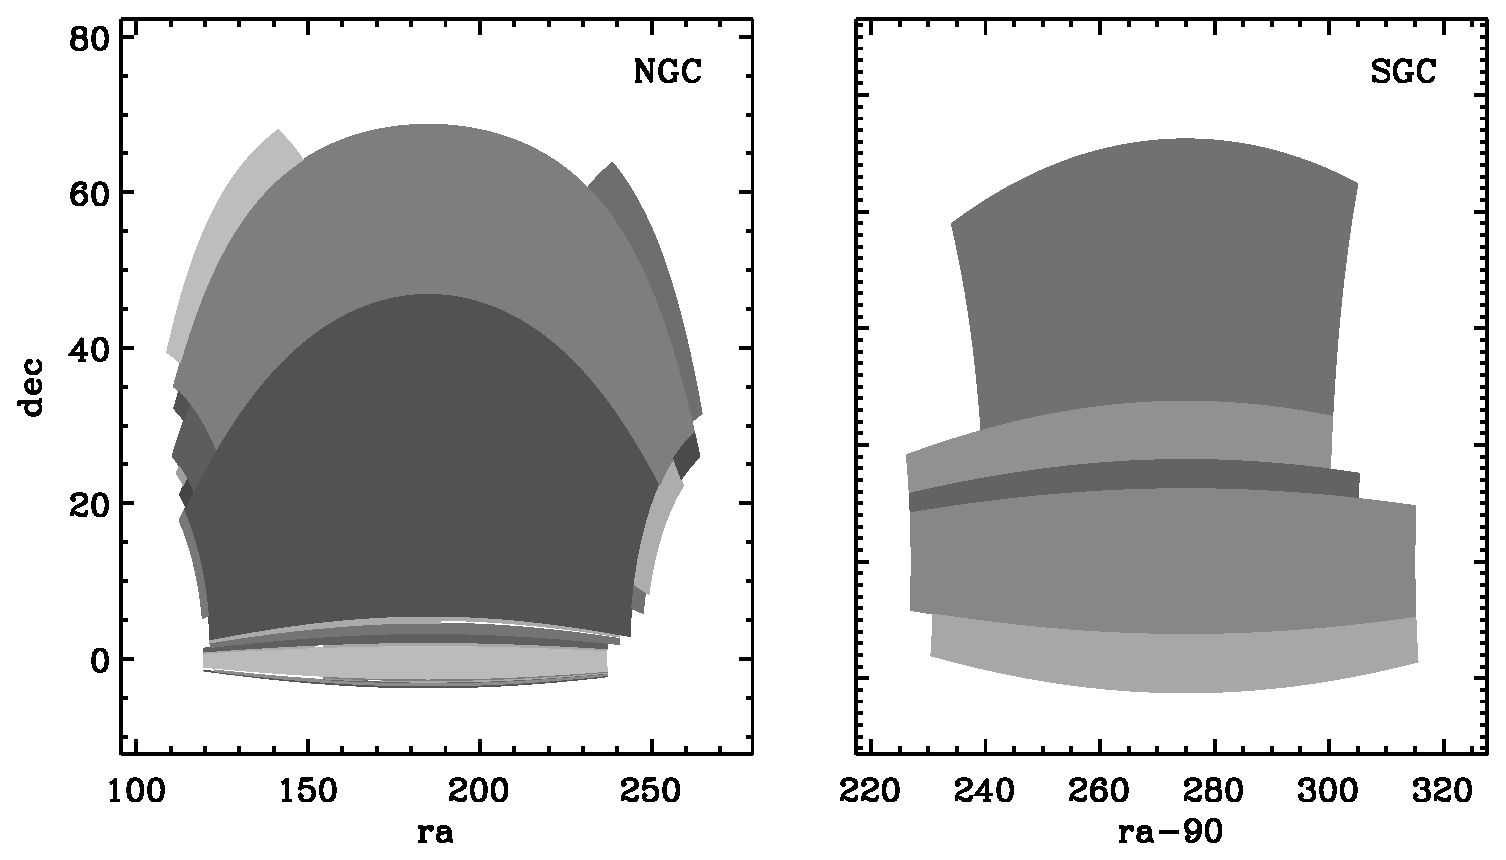
\includegraphics[scale=0.5]{figures/ngc-sgc-poly.eps}
 \caption{BOSS footprint for the north galactic cap on the left
 and the south galactic cap on the right.  The differently shaded
 regions represent contiguous rectangular regions in SDSS survey coordinates.
 Note the plot for the south has been rotated by 90 degrees to avoid
 the split at RA=360. {\color{red} Remake with south wrapping less than zero}}
 \label{fig:footprint}
\end{figure}

The final photometric catalog contains \nphoto\ objects.  The distribution of
extinction corrected \rmag-band \cmodelmag\ and colors derived from extinction
corrected \modelmag\ are shown in \ref{fig:varhist}.

\section{Training Samples} \label{sec:train}

We use a spectroscopic trining set drawn from a number of sources. These
sources contain mostly galaxies and a small number of stars in order to help
characterize stellar contaminants from the photometric sample at low redshift.
In the following sections we give short details on each sample and describe our
process for matching to the photometric sample.

\subsection{Samples Used in this Study} \label{sec:train:def}

\begin{itemize} 

    \item 435,878 redshifts from the SDSS spectroscopic sample,
principally from the \texttt{MAIN} and Luminous Red Galaxy \texttt{(LRG)}
samples, with confidence level \texttt{zconf}$ > 0.9$, and r-band
\cmodelmag\ $ <19.5$.


    \item 412 objects from the Canadian Network for Observational
Cosmology (CNOC) Field Galaxy Survey \cite[CNOC2;][]{yee00}\footnote{\tt
http://www.astro.toronto.edu/~cnoc/cnoc2.html} with \texttt{Rval} $>4$
for \texttt{Sc}$=2$ or \texttt{Rval} $> 5$ for \texttt{Sc}$=5$

    \item 122 from the Canada-France Redshift
Survey \cite[CFRS;][]{lilly95}\footnote{\tt
http://www.oamp.fr/people/tresse/cfrs/cfrs.html} with \texttt{Class} $\geq 3$.

    \item 1,376 from the Deep Extragalact Evolutionary Probe 2 survey
\citep[DEEP2;][]{weiner05}\footnote{\tt http://deep.berkeley.edu/DR3}
with \texttt{zqual} $\geq 3$. 
Of these,1,075 are an approximately magnitude-limited sample from the Extended Groth Strip (EGS).
The remainder is BRI? color-selected to target $z>0.7$ galaxies(hereafter the non-EGS sample). 

    \item 151 from the Team Keck Redshift Survey \cite[TKRS;][]{wirth04}\footnote{\tt http://tkserver.keck.hawaii.edu/tksurvey/}.

    \item 8,577 LRGs from the 2dF-SDSS LRG and QSO Survey \cite[2SLAQ;][]{cannon06}\footnote{\tt http://www.2slaq.info/} with \texttt{qop} $\geq$ 3.

    \item  1,247 from zCOSMOS redshift survey \cite{lilly07}, with  \texttt{cc=3.4 || 3.5 || 4.4.  || 4.5 || 9.5}
    
    \item 1,771 from the VIMOS VLT-Deep survey \cite[VVDS;][]{garilli08}\footnote{\tt http://www.oamp.fr/virmos/vvds.htm} with \texttt{zqual} $\geq 3$.

    \item 14,196 from four fields of the PRIMUS survey \cite[PRIMUS;][]{coil10}\footnote{\tt http://cmb.as.arizona.edu/~eisenste/primus/Home.html}.  Only PRIMUS objects with \texttt{zconf} == 4 were used.      
\end{itemize}


\subsection{Matching to SDSS Imaging Data} \label{sec:train:match}

We match by position the training sets listed in \S \ref{sec:train:def} to the
photometric catalog described in \S \ref{sec:select}.  We choose the closest
match within \matchrad.  By performing this match we place the training set
galaxies on the same photometric system as the photometric set.  We also
guarantee that the matches are drawn from the same magnitude range, and
have the same quality cuts applied, as the photometric set.

As noted in \S \ref{sec:train:def}, the training sets contain some stars.
There are also some stars in the photometric set, since the star galaxy
separation is not perfect.  Thus, through this matching between photometric set
and training set it should be possible to place some fraction of the stars in
the photometric set at redshift zero; or at least some part of their derived
\pofz.

\section{Results}

We use the algorithm described in \S \ref{sec:method} to derive weights for
each training set galaxy.  We then use these weights to calculate a weighted
redshift histogram which, under our assumptions, should be proportional to that
of the training set.  We also derive individual redshift probability
distributions \pofz\ for each photometric galaxy.

The \rmag-band \cmodelmag\ and colors based on \modelmag\ for the photometric
and training sets are shown in figure \ref{fig:varhist}.  Also shown are the
derived weights for the training set and the resulting weighted histograms.
The weighted training set distributions should be approximately proportional to
the photometric set distributions in order to derive good redshift
distributions.  There are deviations at \gmr\ $\sim 1.5$ and \rmi\ $\sim 0.6$,
but otherwise the distributions are quite close.  It may be possible to learn
something by comparing these distributions directly, but we will instead focus
on the accuracy of the recovered redshift distributions.

As detailed in \cite{CunhaPhotoz09}, the weights and P(z) are susceptible to
four kinds of training-set selection effects: spectroscopic failures,
large-scale structure bias (sample variance + shot noise in the training set),
and selection in non-photometric observables.  In addition, the fact that the
weights use a non-infinitesimal volume to re-weight the photometric set can
yield a small Eddington bias to the recovered distribution.  And, as mentioned
previously, incorrect star-galaxy separation can result in incompleteness and
contamination of the sample.  Because our training set consists of many
different surveys with different characteristics, it is important to quantify
the contribution of each to the overall result.  Table \ref{tbl:weistats}
lists, for each of the surveys comprising the training set, the number of
objects, the approximate area, and the percentage the survey contributes to the
weighted estimate of the overall redshift distribution.  This percentage is
calculated by summing up the weights assigned to objects in each survey and
dividing by the sum of weights from the entire training set.


From Table \ref{tbl:weistats}, we see that PRIMUS carries the most weight by a
large margin at 62\%.  Overall, the magnitude limited surveys that reach our
our selection depth of \rmax\ - PRIMUS, TKRS, CNOC2, DEEP2-EGS, CFRS, VVDS, and
zCOSMOS - represent about 81$\%$ of the total weight.  This is desirable,
because it minimizes the risk of bias in our assessment errors in what follows.

\begin{itemize}

\item {\it Large-scale structure:} We expect this to be the main source of
error.  We use galaxy+n-body simulations\footnote{courtesy of Risa Wechsler and
Michael Busha, private communication} to estimate the sample variance plus shot
noise uncertainties of the spectroscopic redshift distributions of the training
set.  For simplicity, we only simulate the magnitude limited surveys of the
training set.  In addition, because of the overlap between zCOSMOS and one of
the PRIMUS fields, we neglect the zCOSMOS sample in the error estimation to
simplify the calculation.  This results in a $\sim$10\% increase in the error
bars relative to including zCOSMOS as an independent sample.  The predicted
error bars are overlayed on the simulated overall redshift distribution in Fig.
\ref{fig:ebars}.  The uncertainty in the training set redshift distributions is
not identical to that of the uncertainties in the estimated redshift
distributions N(z) derived using the weights, hence the error bars should be
used only for a reasonable reference.  A more detailed estimation of the errors
would require SDSS specific photometry+n-body simulations.  Relative to the
error bars in the training set, the error bars in the weighted N(z) is about
20-30\% smaller, but this requires more detailed investigation.  There are also
significant anti-correlations between neighboring bins in the weighted redshift
distribution.  We will explore these issues in more detail in
\citet{CunhaPhotozLSS11}.

\item {\it Selection in non-observables:} Two of the surveys comprising our
training set have selections in observables that are not included in the SDSS
magnitude limited sample.  As mentioned previously, the DEEP2-nonEGS sample is
selected using BRI photometry to target galaxies above $z>0.7$.  As shown in
\citet{CunhaPhotoz09}, the use of DEEP2 in earlier versions of this catalog
would cause a bump in the overall estimated redshift distribution around $z\sim
0.8$.  The more recent data release has a brighter magnitude cut and additional
data, and these issues have largely been eliminated this bias.  Note
DEEP2-nonEGS carries about 2.7\% of the total weight.  The 2SLAQ sample targets
LRG's.  Besides SDSS magnitudes, it also uses morphological information in the
selection.  Because shape correlates poorly with redshift, biases due to the
2SLAQ sample are expected to be small.  2SLAQ is an important part of our
sample because it provides a good training set for LRG's at higher redshift
than the SDSS sample.

\item {\it Spectroscopic failures} The impact of spectroscopic failures is the
most difficult to quantify.  We chose a bright r-magnitude cut, and relatively
stringent cuts on spectroscopic quality to minimize effects of failures, but it
is possible that some features seen in the redshift distribution - such as the
dip around $z=0.4$ are due partly to spectroscopic failures.
{\color{red} this seems speculative, can we say anything quantitative?  If not
perhaps simplify the comment to ``it is possible that there are significant
errors due to spectroscopic failures''.}

\item {\it Star-galaxy separation? Discuss it here or somewhere else? {\color{red} I'm
looking into the expected contamination.  It's OK of course if there are stars as long as they
pile up at zero redshift!}}

\end{itemize}

\begin{figure}[t]\centering
    \includegraphics[{angle = -90,scale=0.4}]{figures/nz.sim.error.ps}
    \caption{\color{red}{This seems fine; we need a caption}}
    \label{fig:ebars}

    \vspace{2em}
\end{figure}

%}

\begin{table}[!ht]
\caption{{\color{red}We should use deluxetable and add a caption}}
\label{tbl:weistats}
\begin{center}
\begin{tabular}{ l r r r }\hline \hline
Survey & Number of objects & Area$deg^2$ & Weight fraction \\ \hline 
PRIMUS$^*$ &14,196 &5.2 & 62\% \\
2SLAQ  &8,577 & 180 & 7.0\%\\
TKRS$^*$  &151  & 0.07& 0.50\%\\
CNOC2$^*$ &412  &0.4 & 1.8\%\\
DEEP2-EGS$^{*!}$ &1,075  & 0.4 & 3.5\%\\
DEEP2-nonEGS$^{*!}$ &301  & 2.8 & 2.7\%\\
SDSS &435,878  & & 9.1\%\\
CFRS$^*$ &122  & $<$0.1 & 0.67\%\\
VVDS$^*$ &1,771  &4.0  & 5.5\%\\
zCOSMOS$^*$ &1,247 &1.7  & 7.4\% \\ \hline \hline
 %\multicolumn{2}{c |}{Survey} & \multicolumn{2}{| c}{Parameter Uncertainty} \\ \hline
%Original Parameters & New Parameters & $\sigma(\DE)$ & $\sigma(w)$ \\ \hline
%free & free & 0.8662 & 0.4206 \\
%\multicolumn{2}{l}{add Planck priors} & 0.0331 & 0.1078 \\
%\multicolumn{2}{l}{Planck priors} & 0.0331 & 0.1078 \\
%free & sharp & 0.0142 & 0.0456 \\
%sharp & sharp & 0.0024 & 0.0110 \\ \hline
\end{tabular}
\end{center} 
\end{table}


\cc{=============================} 

\begin{figure}[t] \centering
    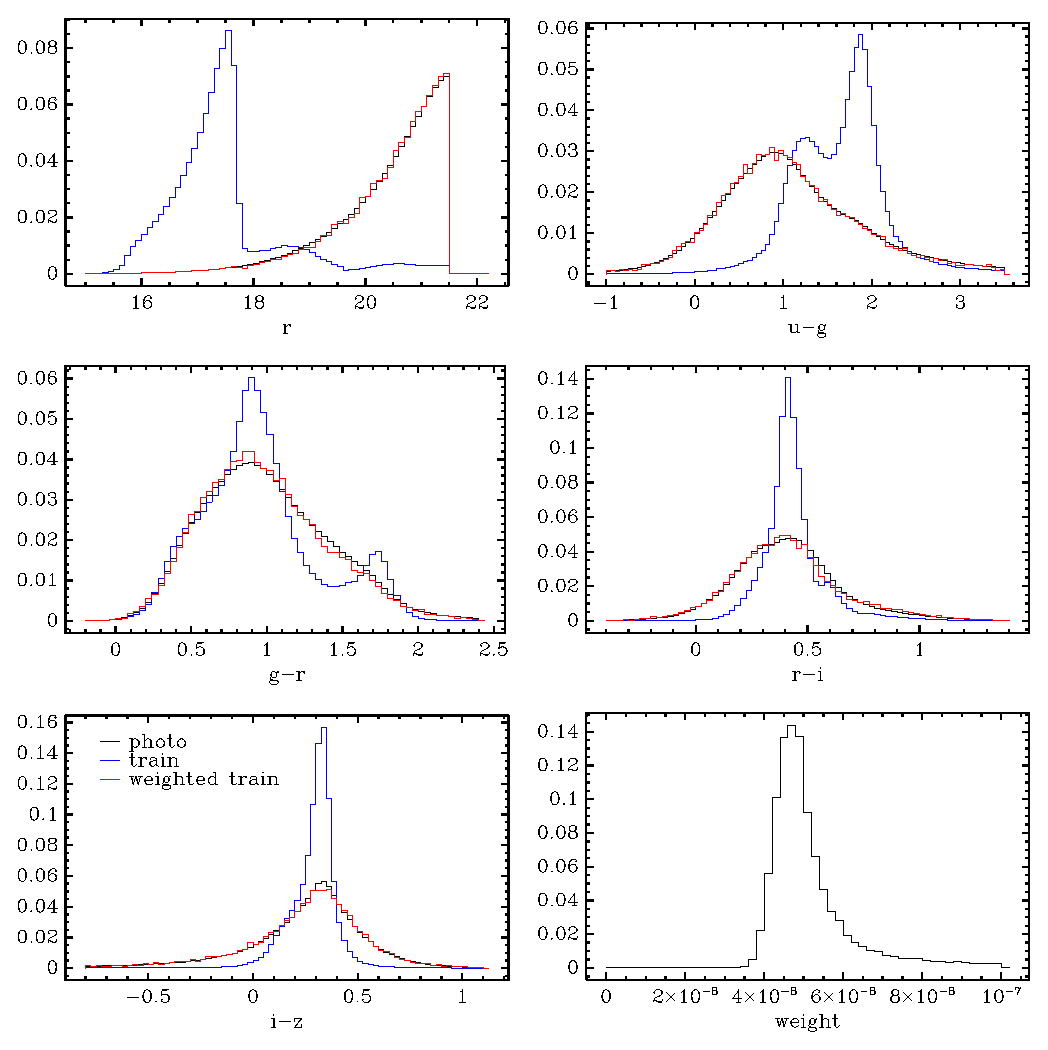
\includegraphics{figures/zweight-09-varhist.eps}

    \caption{Distributions of photometric quantities for the photometric sample
    and training sample.  The upper left panel shows the extinction-corrected
    \rmag-band \cmodelmag.  Note both samples are cut at \rmag$ < $\rmax.  
    Also shown is the weighted histogram for the training sample where
    the weights are derived to produced distributions approximately 
    proportional to the photometric sample.
    The following four panels show extinction corrected colors based on
    \modelmag.  The bottom right panel shows the distribution of of the
    derived weights for the training sample. {\color{red} replace with 21.8?}}
    \label{fig:varhist}

    \vspace{2em}
\end{figure}

Figure \ref{fig:pofz} shows the recovered redshift distribution for the entire
\rmag\ $<$ \rmax\ sample.  Also shown is the redshift distribution of the
original training set.  These distributions are in qualitative agreement with
those shown in \citet{CunhaPhotoz09}, although that sample had a fainter \rmag\
limit at 22.0.  Note the sub-plot showing the region near $z=0$.  As expected
there is some fraction of the overall distribution near z=0.  The fraction of
at $z < 0.002$ is about 0.4\%.  It is not known exactly how many stars are in
the photometric sample, but this is probably a lower limit on the stellar
contamination {\color{red}beef this up}.

Also shown in \ref{fig:pofz} is the summed \pofz\ derived for individual
galaxies.  The summed \pofz\ favors lower redshift than the overall weighted
redshift histogram, although the expectation value of the redshift is within a
percent {\color{red} Carlos what was the number?}.  This is suggestive that
these individual \pofz\ can be used meaningfully on their own. {\color{red} 
we need some estimates of the bias for both approaches here.  If we are
skipping rachel's stuff then we need an alternative.}

\begin{figure}[t] \centering
    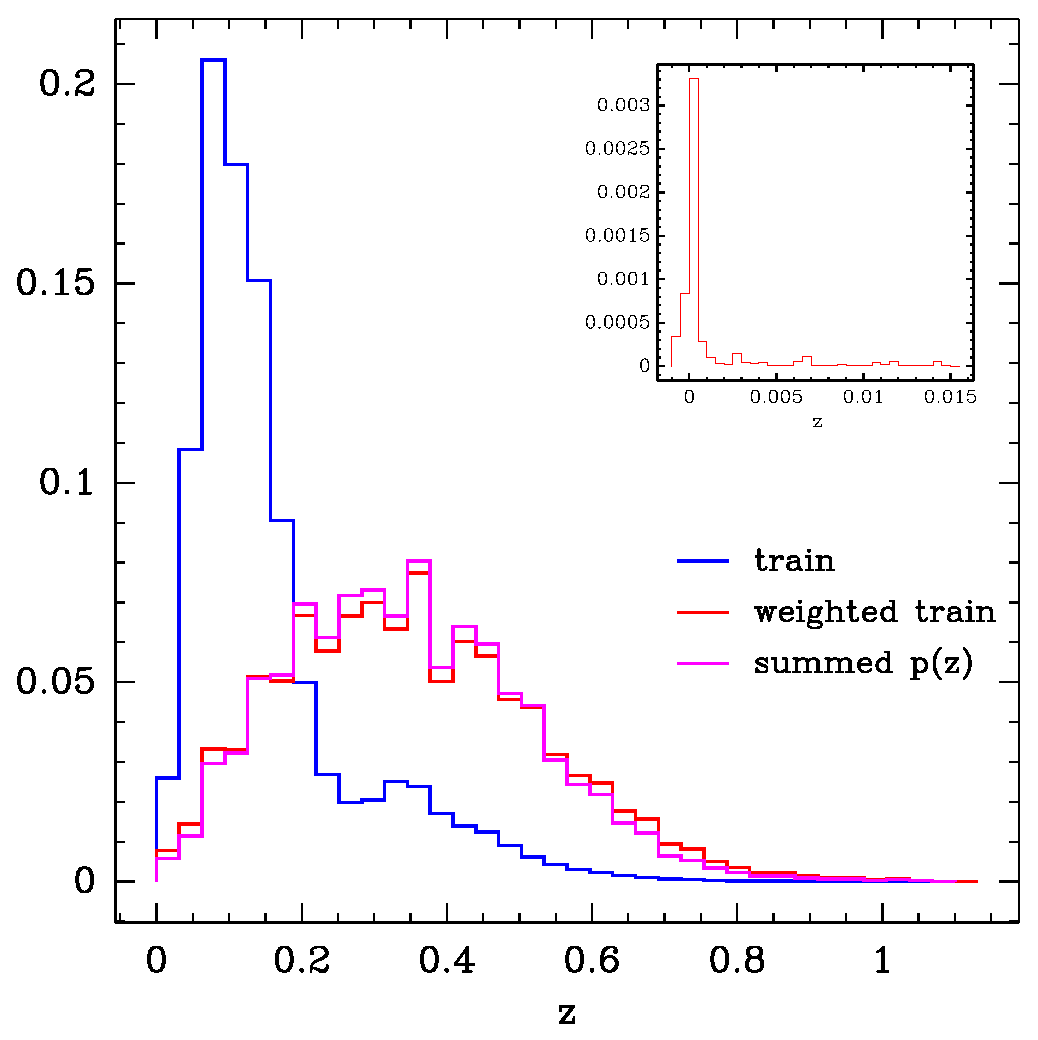
\includegraphics[scale=0.9]{figures/zweight-09-zhist-withorig-withsum-11.eps}

    \caption{Reconstructed redshift distribution for SDSS galaxies with \rmag\
    $ < $ \rmax.  The overall reconstructed distribution, shown in red, is
    derived by creating a weighted histogram of the training set redshifts as
    described in the text.  Also shown in magenta is the sum of all \pofz\
    derived for individual galaxies.  The unweighted training set redshift
    distribution is shown in blue.  The excess at $z \sim 0$ is due to stars in
    training set having signifcant weight; more detail at low redshift is shown
    in the inset.  This excess is at least partly due to the presence of real
    stars in our photometric sample resulting from imperfect star-galaxy
    separation.  The fraction of the distribution at $z < 0.002$ is 0.4\%,
    which is probably a lower bound on the stellar contamination.
    \label{fig:pofz}}

    \vspace{2em}
\end{figure}

The uncertainty in individual p(z)'s is typically dominated by shot-noise
error.  The scale of both statistical and systematic uncertainties in the
individual $p(z)$'s are strongly correlated with the width of the $p(z)$
{\color{red} can we show this here or will we just reference your other
paper?}.  Fig.  \ref{fig:pzwidth} shows the distribution of objects in the
photometric sample as a function of r-band magnitude and $1-\sigma$ width of
the $p(z)$.  The contours indicate factor of 2 changes in density.  

We recommend using the $1-\sigma$ or other width measures of the $p(z)$ as the
most efficient way to trim the sample for improved precision and accuracy.  The
$p(z)$ width should also be a reasonable error estimator for use with other
photo-z methods.  However, we discourage using the peak or some other single
number statistic derived from the $p(z)$ as a proxy for redshift. See 
\S \ref{sec:usage} for more details.
\begin{comment} If a single-number photo-z estimate is needed we recommend
using a neural network or nearest-neighbor polynomial based approach
\cite[e.g.][]{Oyaizu08}.  \end{comment}

\begin{figure}[!t]\centering
    \includegraphics[scale=0.25]{figures/pzwidth.ps}
    \caption{\textcolor{blue}{This is just a placeholder plot. It needs many improvements.}}
    \label{fig:pzwidth}

    \vspace{2em}
\end{figure}

\section{Proper Usage} \label{sec:usage}

If one desires to use the $P(z)$ to evaluate any lin-linear function $F(z)$,
one must integrate over the entire distribution; i.e. one must take the
expectation value.  The reason is quite simple. In general the following
relation holds:
\begin{equation}
\langle F(z) \rangle \ne F(\langle z \rangle).
\end{equation}
The expectation value is computed as follows:
\begin{equation}
\langle F \rangle = \int_{0}^{\infty} F(z) P(z) dz.
\end{equation}
It is {\bf not} correct to simply take the mean of $P(z)$ and use it to evaluate
a function.

This is true in most interesting science cases.  An excellent example is in
gravitational lensing, where one must estimate the ``critical density for
lensing'' $\Sigma_{crit}$.  The function $\Sigma_{crit}$ depends in a highly
non-linear way on the angular diameters to lens, source and between lens and
source.  The proper estimator for a lens at redshift $z_{l}$ and source with
$P(z_s)$ is
\begin{equation}
\Sigma_{crit}(z_l) = \int_{0}^{\infty} \Sigma_{crit}(z_l, z_s) P(z_s) dz_s.
\end{equation}

\bibliographystyle{apj}
% Bib database
\bibliography{apj-jour,astroref}



\end{document}

